% DiCE LGBM
\begin{table}
\centering
\begin{tabular}{lcccc}
\toprule
\textbf{Instancia} & \textbf{spectral flatness} & \textbf{mfcc 1} & \textbf{mfcc 5} & \textbf{Etiqueta} \\
\midrule
Explicada & 0.11064 & -330.39648 & 6.07202 & 0 \\
Counter factual 1 & 0.01700 &  &  & 1 \\
Counter factual 2 & 0.02708 & -382.50071 &  & 1 \\
Counter factual 3 & 0.02945 &  & 13.43934 & 1 \\
\bottomrule
\end{tabular}
\caption{Counter factuals generados por DiCE para LightGBM}
\label{tab:dice_lgbm}
\end{table}

% resultatos SVM sin spectral flatness
\begin{table}
\centering
\begin{tabular}{lc}
\toprule
\textbf{Métrica} & \textbf{Valor}\\
\midrule
Accuracy & 1 \\
Precision & 1 \\
Recall & 1 \\
F1-Score & 1  \\
AUC-ROC & 1 \\
MCC & 1 \\ 
\bottomrule
\end{tabular}
\caption{Métricas principales de SVM sin spectral flatness}
\label{tab:metricas_principales_svm_sin_specflat}
\end{table}

\begin{table}
\centering
\begin{tabular}{lcccc}
\toprule
\textbf{Dato} & \textbf{Precisión} & \textbf{Recall} & \textbf{F1-Score} & \textbf{Nº Instancias} \\
\midrule
Real (1) & 1.0000 & 1.0000 & 1.0000 & 10 \\
IA (0) & 1.0000 & 1.0000 & 1.0000 & 10 \\
accuracy &  &  & 1.0000 & 20 \\
macro avg & 1.0000 & 1.0000 & 1.0000 & 20 \\
weighted avg & 1.0000 & 1.0000 & 1.0000 & 20 \\
\bottomrule
\end{tabular}
\caption{Classification report de SVM sin spectral flatness}
\label{tab:classification_report_svm_sin_specflat}
\end{table}

\begin{table}
\centering
\begin{tabular}{lc}
\toprule
\textbf{Tipo de predicción} & \textbf{Cantidad}\\
\midrule
Verdaderos Negativos & 10 \\
Verdaderos Positivos & 10 \\
Falsos Positivos & 0 \\
Falsos Negativos & 0  \\
Error tipo I & 0\% \\
Error tipo II & 0\% \\ 
\bottomrule
\end{tabular}
\caption{Análisis de errores de SVM sin spectral flatness}
\label{tab:analisis_errores_svm_sin_specflat}
\end{table}

% SHAP SVM sin spectral flatness
\begin{figure}
	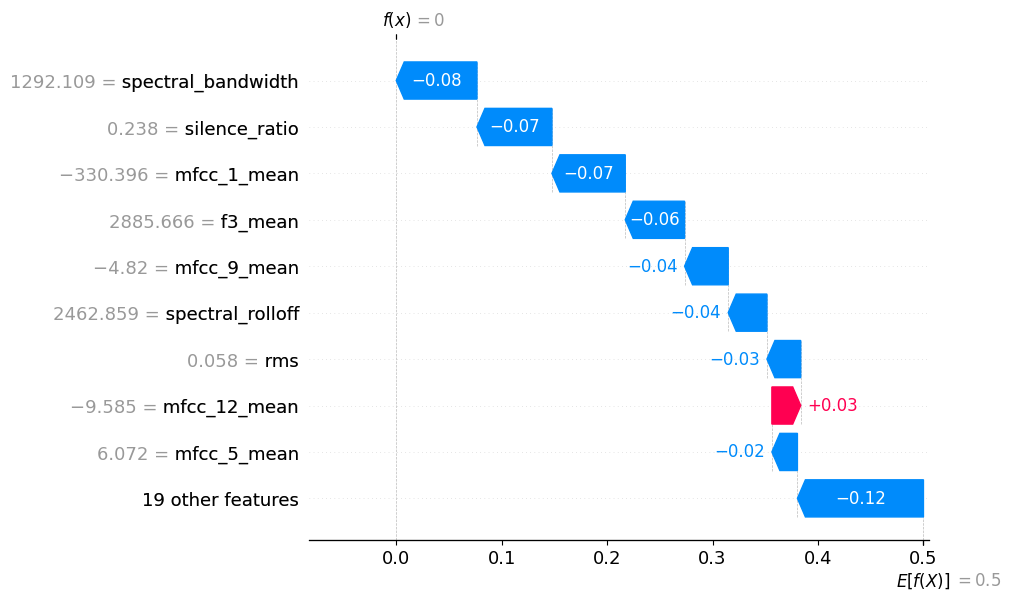
\includegraphics[width=\textwidth]{imagenes/shap_svm_sin_specflat_1.png}
	\caption{Explicación local de SVM con SHAP tras quitar spectral flatness}
	\label{fig:1_shap_svm_local_sin_specflat}
\end{figure}

\begin{figure}
	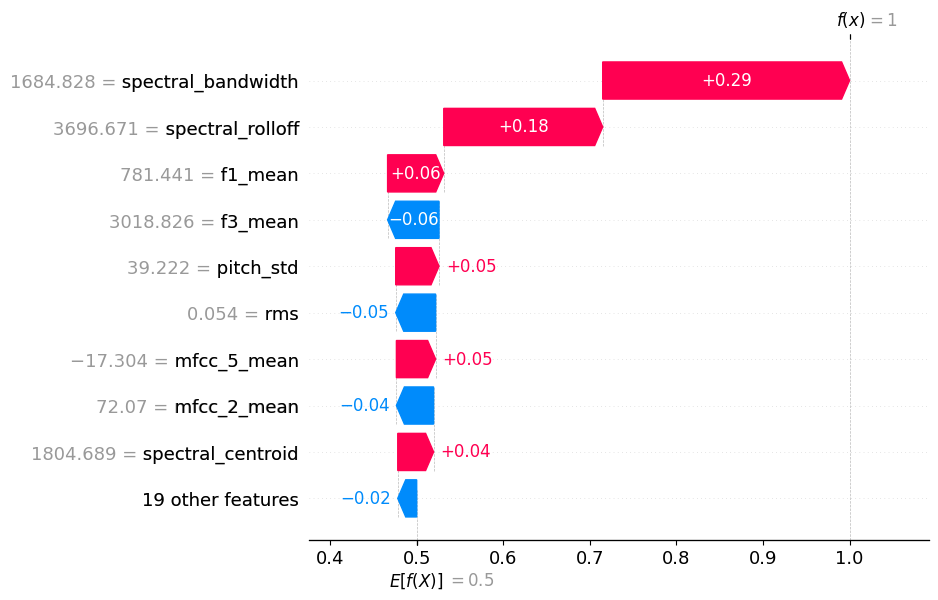
\includegraphics[width=\textwidth]{imagenes/shap_svm_sin_specflat_2.png}
	\caption{Explicación local de SVM con SHAP tras quitar spectral flatness}
	\label{fig:2_shap_svm_local_sin_specflat}
\end{figure}

% resultados SVM sin spectral flatness, mfcc 1 y spectral bandwidth
\begin{table}
\centering
\begin{tabular}{lc}
\toprule
\textbf{Métrica} & \textbf{Valor}\\
\midrule
Accuracy & 1 \\
Precision & 1 \\
Recall & 1 \\
F1-Score & 1  \\
AUC-ROC & 1 \\
MCC & 1 \\ 
\bottomrule
\end{tabular}
\caption{Métricas principales de SVM sin spectral flatness, mfcc1 y spectral bandwidth}
\label{tab:metricas_principales_svm_sin_sflat_mfcc1_sband}
\end{table}

\begin{table}
\centering
\begin{tabular}{lcccc}
\toprule
\textbf{Dato} & \textbf{Precisión} & \textbf{Recall} & \textbf{F1-Score} & \textbf{Nº Instancias} \\
\midrule
Real (1) & 1.0000 & 1.0000 & 1.0000 & 10 \\
IA (0) & 1.0000 & 1.0000 & 1.0000 & 10 \\
accuracy &  &  & 1.0000 & 20 \\
macro avg & 1.0000 & 1.0000 & 1.0000 & 20 \\
weighted avg & 1.0000 & 1.0000 & 1.0000 & 20 \\
\bottomrule
\end{tabular}
\caption{Classification report de SVM sin spectral flatness, mfcc1 y spectral bandwidth}
\label{tab:classification_report_svm_sin_sflat_mfcc1_sband}
\end{table}

\begin{table}
\centering
\begin{tabular}{lc}
\toprule
\textbf{Tipo de predicción} & \textbf{Cantidad}\\
\midrule
Verdaderos Negativos & 10 \\
Verdaderos Positivos & 10 \\
Falsos Positivos & 0 \\
Falsos Negativos & 0  \\
Error tipo I & 0\% \\
Error tipo II & 0\% \\ 
\bottomrule
\end{tabular}
\caption{Análisis de errores de SVM sin spectral flatness, mfcc1 y spectral bandwidth}
\label{tab:analisis_errores_svm_sin_sflat_mfcc1_sband}
\end{table}

% SHAP SVM sin spectral flatness, mfcc 1 y spectral bandwidth
\begin{figure}
	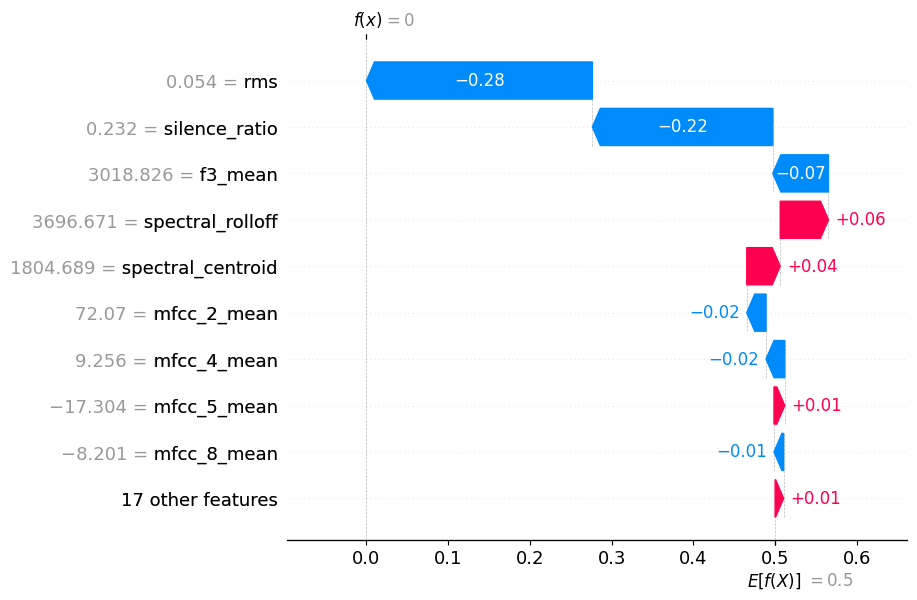
\includegraphics[width=\textwidth]{imagenes/shap_svm_sin_sflat_mfcc1_sband_1.png}
	\caption{Explicación local de SVM con SHAP tras quitar spectral flatness, mfcc 1 y spectral bandwidth}
	\label{fig:1_shap_svm_local_sin_sflat_mfcc1_sband}
\end{figure}

\begin{figure}
	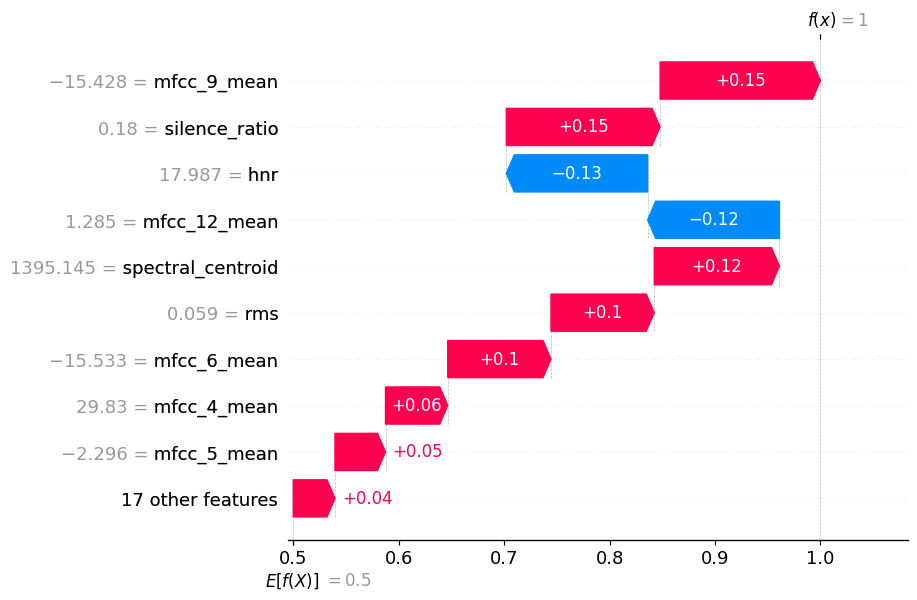
\includegraphics[width=\textwidth]{imagenes/shap_svm_sin_sflat_mfcc1_sband_2.png}
	\caption{Explicación local de SVM con SHAP tras quitar spectral flatness, mfcc 1 y spectral bandwidth}
	\label{fig:2_shap_svm_local_sin_sflat_mfcc1_sband}
\end{figure}

% LIME SVM
\begin{figure}
	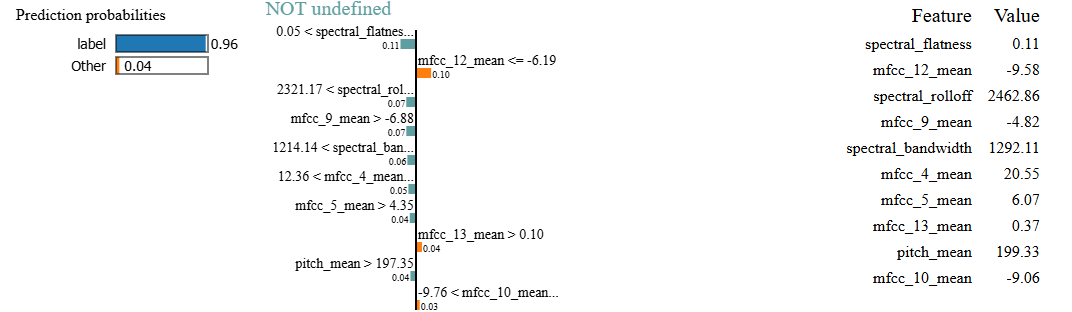
\includegraphics[width=\textwidth]{imagenes/lime_svm.png}
	\caption{Explicación local de SVM con LIME}
	\label{fig:lime_svm}
\end{figure}

% Pipe RF SHAP local
\begin{figure}
	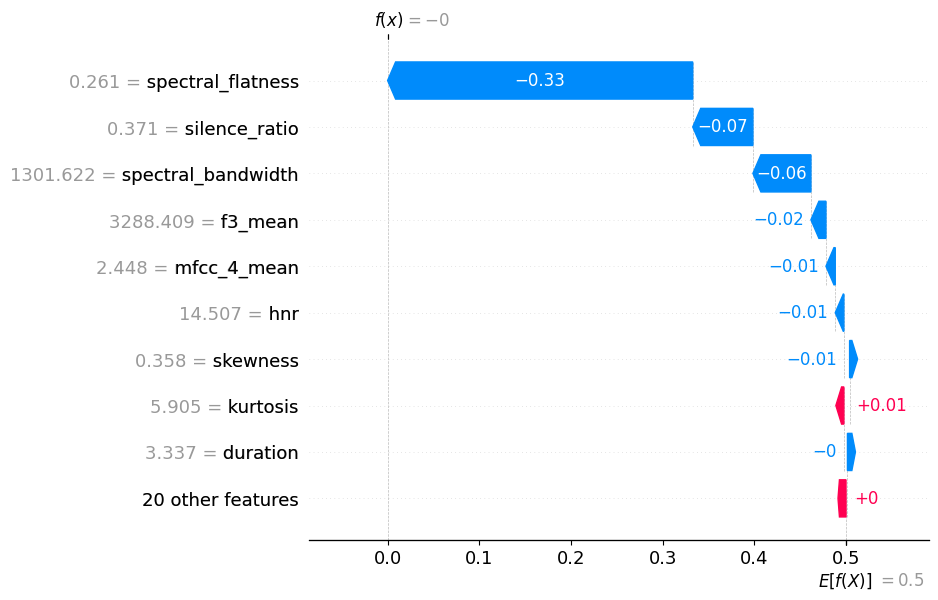
\includegraphics[width=\textwidth]{imagenes/pipe_shap_rf_local_1.png}
	\caption{Explicación local de RF con SHAP para audios nuevos en español}
	\label{fig:pipe_shap_rf_esp_1}
\end{figure}

\begin{figure}
	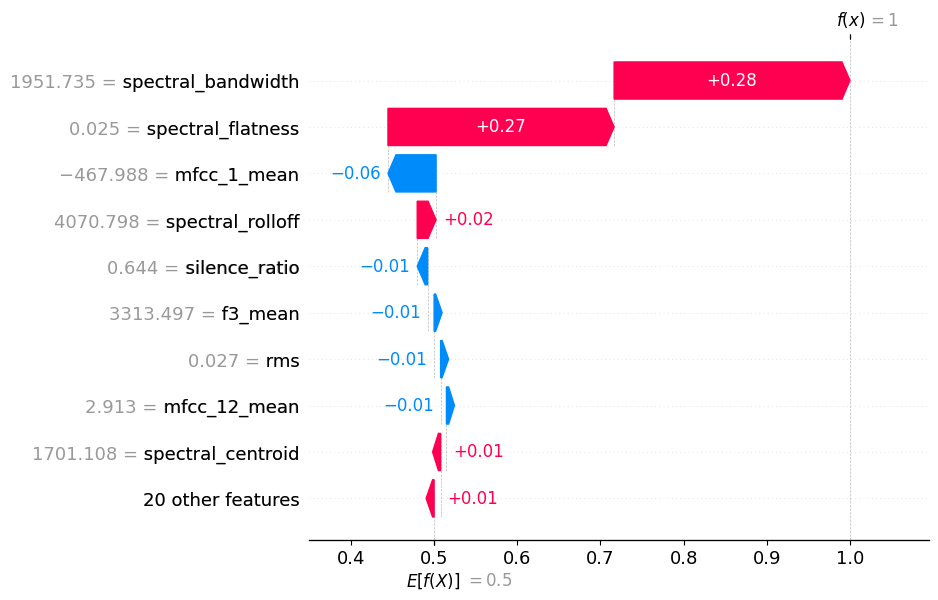
\includegraphics[width=\textwidth]{imagenes/pipe_shap_rf_local_2.png}
	\caption{Explicación local de RF con SHAP para audios nuevos en español}
	\label{fig:pipe_shap_rf_esp_2}
\end{figure}

% Pipe RF SHAP local ingles
\begin{figure}
	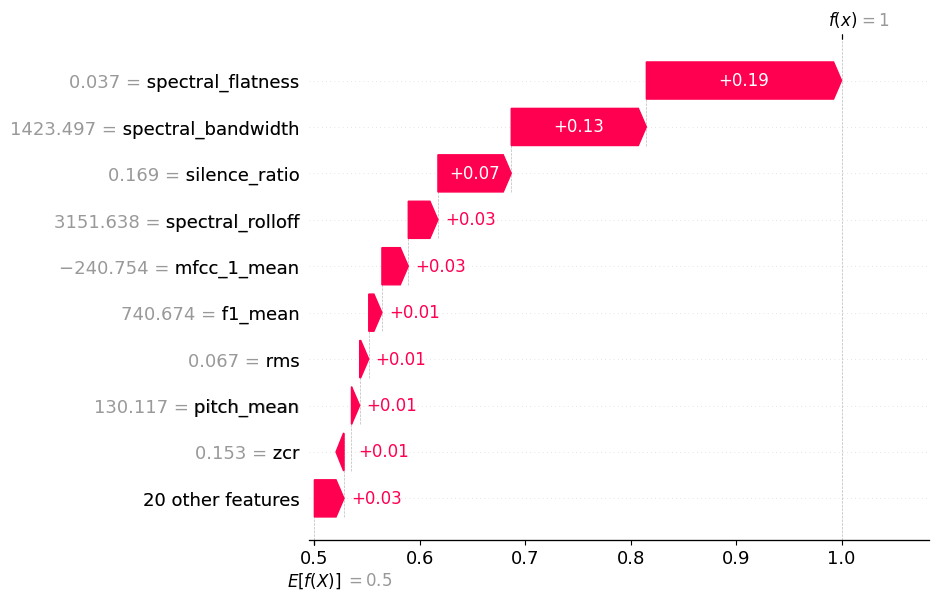
\includegraphics[width=\textwidth]{imagenes/pipe_shap_rf_local_eng_1.png}
	\caption{Explicación local de RF con SHAP para audios nuevos en inglés}
	\label{fig:pipe_shap_rf_eng_1}
\end{figure}

\begin{figure}
	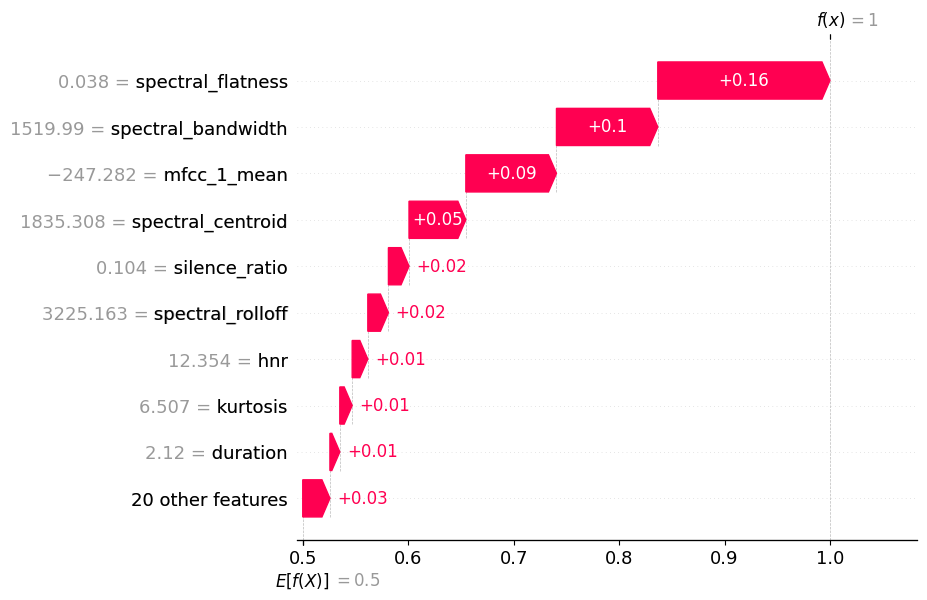
\includegraphics[width=\textwidth]{imagenes/pipe_shap_rf_local_eng_2.png}
	\caption{Explicación local de RF con SHAP para audios nuevos en inglés}
	\label{fig:pipe_shap_rf_eng_2}
\end{figure}

% Pipe RF SHAP global
\begin{figure}
	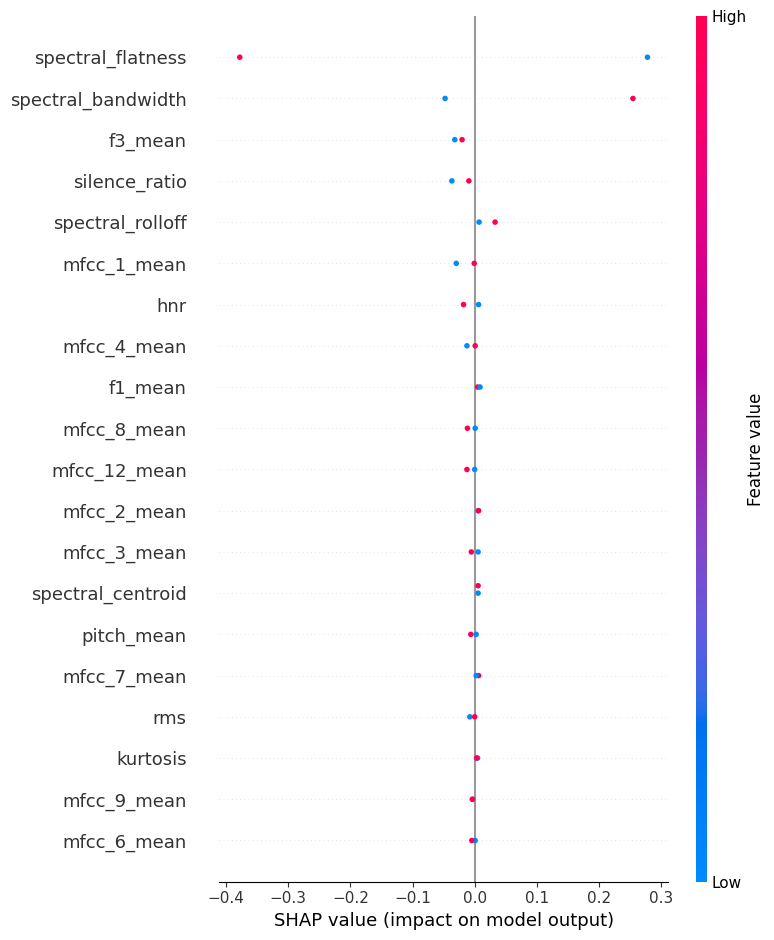
\includegraphics[width=\textwidth]{imagenes/pipe_shap_rf_global.png}
	\caption{Explicación global de RF con SHAP}
	\label{fig:pipe_shap_rf_global}
\end{figure}

% Pipe RF LIME
\begin{figure}
	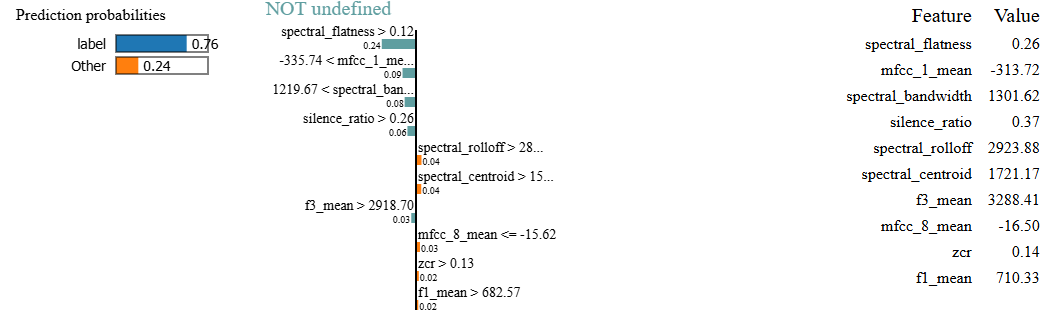
\includegraphics[width=\textwidth]{imagenes/pipe_lime_rf.png}
	\caption{Explicación local de RF con LIME}
	\label{fig:pipe_lime_rf}
\end{figure}

% Pipe RF DiCE
\begin{table}
\centering
\begin{tabular}{lccccc}
\toprule
\textbf{Instancia} & \textbf{spectral flatness} & \textbf{f2} & \textbf{mfcc 3} & \textbf{mfcc 12} & \textbf{Etiqueta} \\
\midrule
Explicada & 3.30119 & 0.25782 & -0.66065 & -0.95448 & 0 \\
Counter factual 1 & -0.87350 &  & 2.60367 &  & 1 \\
Counter factual 2 & -0.01860 & 1.30719 &  &  & 1 \\
Counter factual 3 & -0.09155 &  &  & -2.39793 & 1 \\
\bottomrule
\end{tabular}
\caption{Counter factuals generados por DiCE para RF con audios nuevos}
\label{tab:pipe_dice_rf}
\end{table}

% Pipe LGBM SHAP local
\begin{figure}
	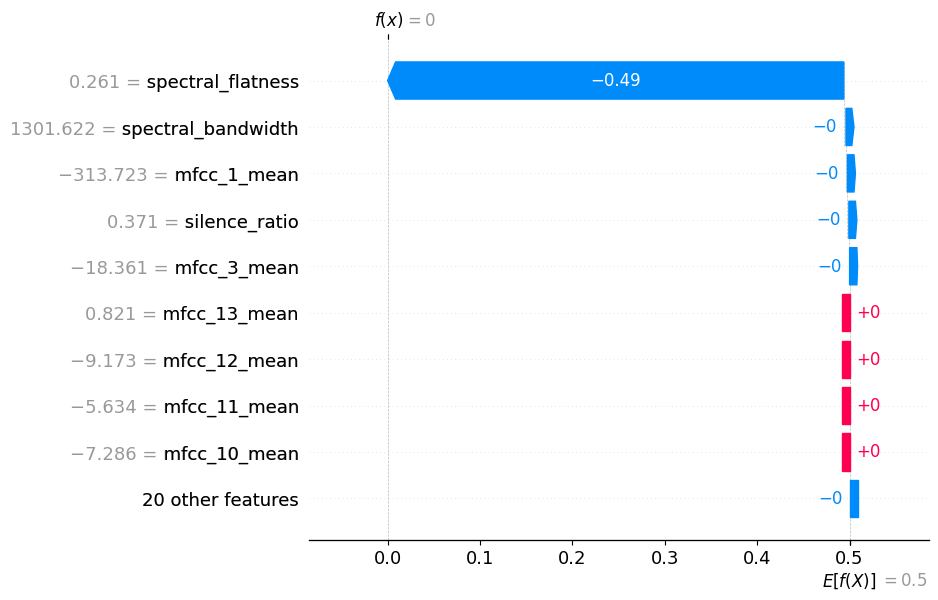
\includegraphics[width=\textwidth]{imagenes/pipe_shap_lgbm_local_1.png}
	\caption{Explicación local de LGBM con SHAP para audios nuevos en español}
	\label{fig:pipe_shap_lgbm_esp_1}
\end{figure}

\begin{figure}
	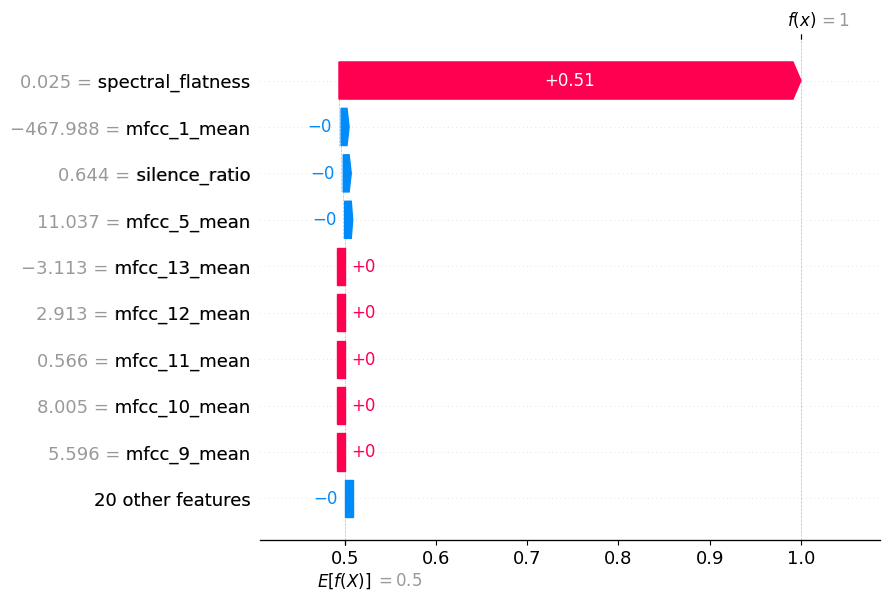
\includegraphics[width=\textwidth]{imagenes/pipe_shap_lgbm_local_2.png}
	\caption{Explicación local de LGBM con SHAP para audios nuevos en español}
	\label{fig:pipe_shap_lgbm_esp_2}
\end{figure}

% Pipe LGBM SHAP local ingles
\begin{figure}
	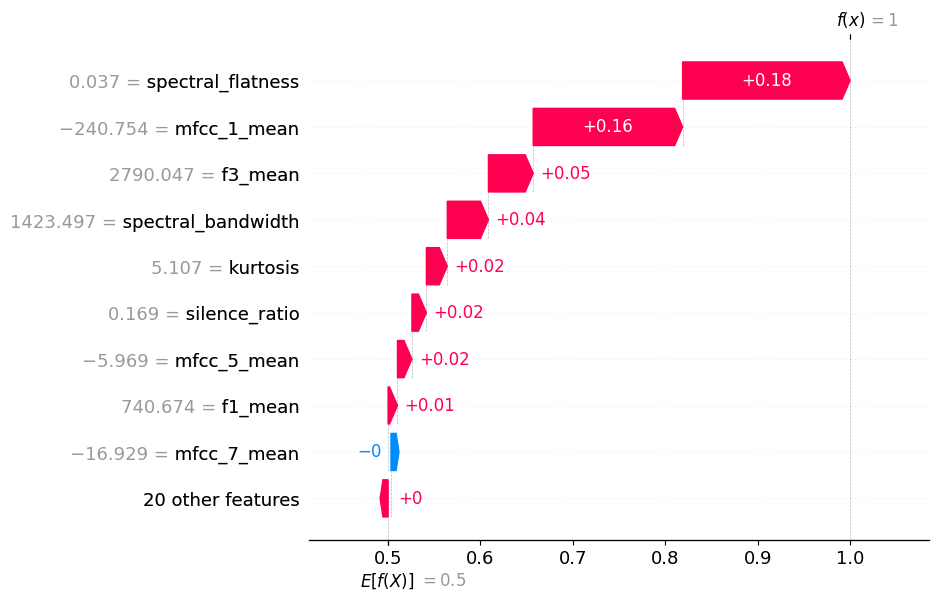
\includegraphics[width=\textwidth]{imagenes/pipe_shap_lgbm_local_eng_1.png}
	\caption{Explicación local de LGBM con SHAP para audios nuevos en inglés}
	\label{fig:pipe_shap_lgbm_eng_1}
\end{figure}

\begin{figure}
	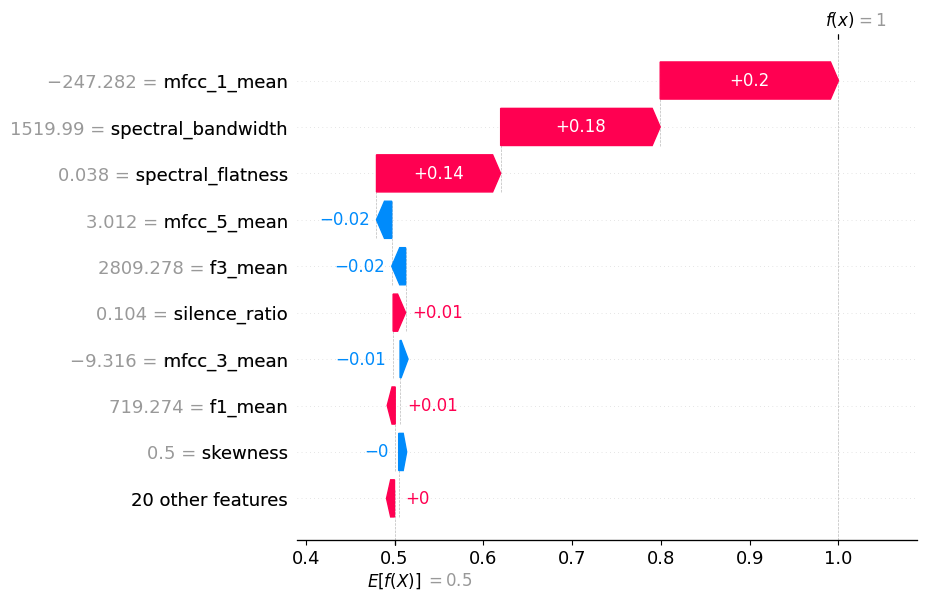
\includegraphics[width=\textwidth]{imagenes/pipe_shap_lgbm_local_eng_2.png}
	\caption{Explicación local de LGBM con SHAP para audios nuevos en inglés}
	\label{fig:pipe_shap_lgbm_eng_2}
\end{figure}

% Pipe LGBM SHAP global
\begin{figure}
	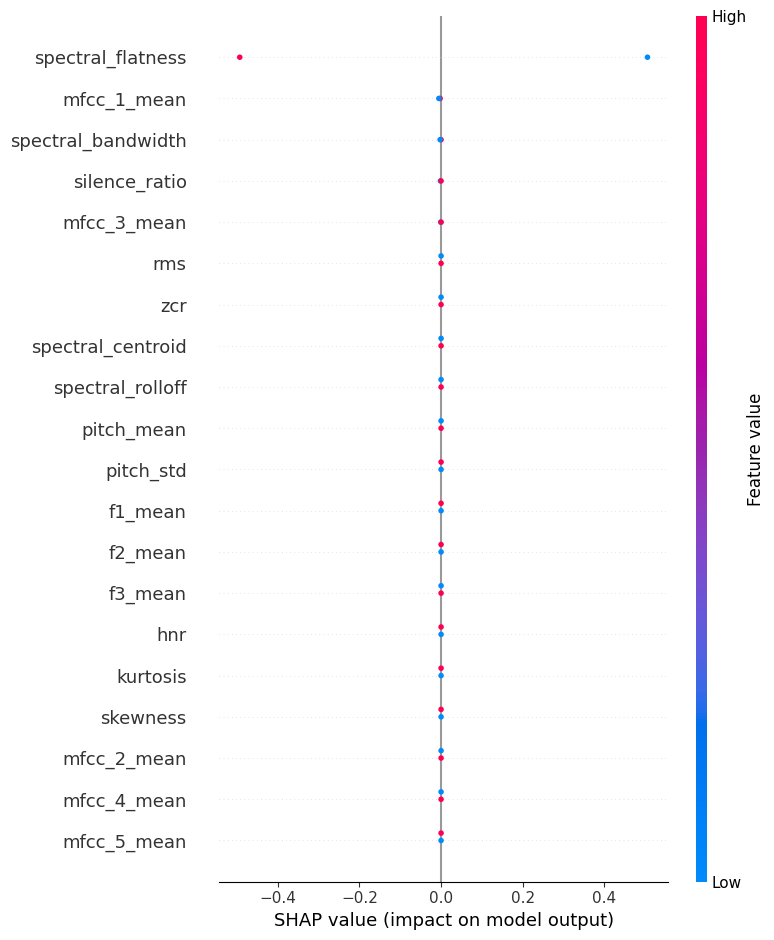
\includegraphics[width=\textwidth]{imagenes/pipe_shap_lgbm_global.png}
	\caption{Explicación global de LGBM con SHAP}
	\label{fig:pipe_shap_lgbm_global}
\end{figure}

% Pipe LGBM LIME
\begin{figure}
	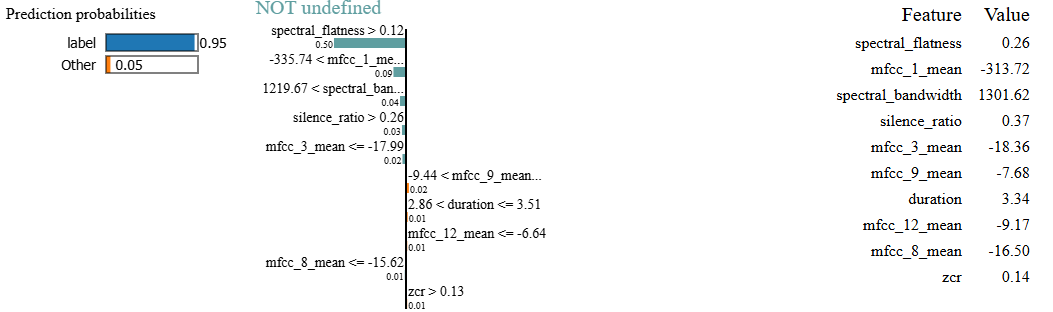
\includegraphics[width=\textwidth]{imagenes/pipe_lime_lgbm.png}
	\caption{Explicación local de LGBM con LIME}
	\label{fig:pipe_lime_lgbm}
\end{figure}

% Pipe LGBM DiCE
\begin{table}
\centering
\begin{tabular}{lccc}
\toprule
\textbf{Instancia} & \textbf{spectral flatness} & \textbf{mfcc 4} & \textbf{Etiqueta} \\
\midrule
Explicada & 3.30119 & -1.61693 & 0 \\
Counter factual 1 & -0.23885 &  & 1 \\
Counter factual 2 & -0.77720 &  & 1 \\
Counter factual 3 & -0.75138 & -2.12114 & 1 \\
\bottomrule
\end{tabular}
\caption{Counter factuals generados por DiCE para RF con audios nuevos}
\label{tab:pipe_dice_lgbm}
\end{table}

% Pipe SVM SHAP local
\begin{figure}
	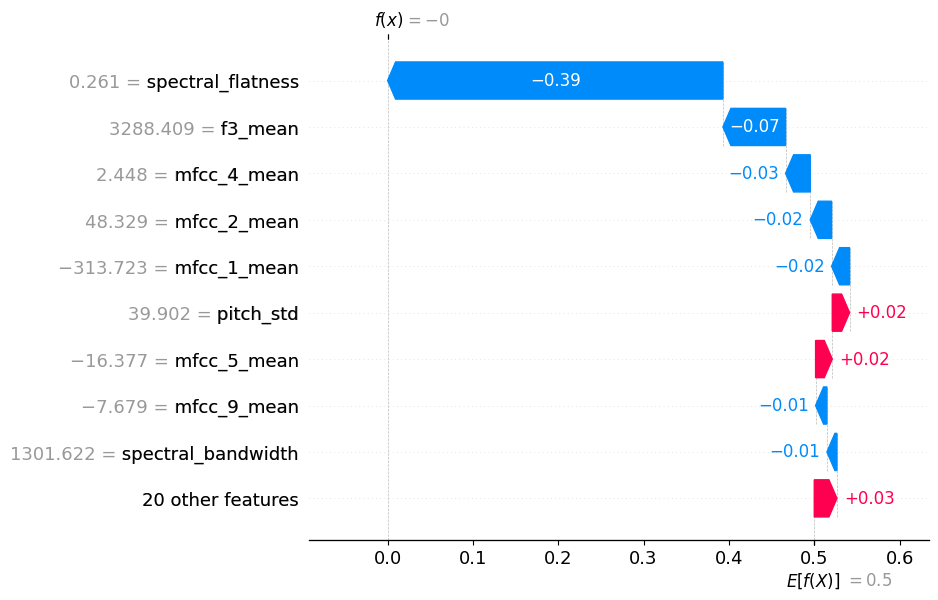
\includegraphics[width=\textwidth]{imagenes/pipe_shap_svm_local_1.png}
	\caption{Explicación local de SVM con SHAP para audios nuevos en español}
	\label{fig:pipe_shap_svm_esp_1}
\end{figure}

\begin{figure}
	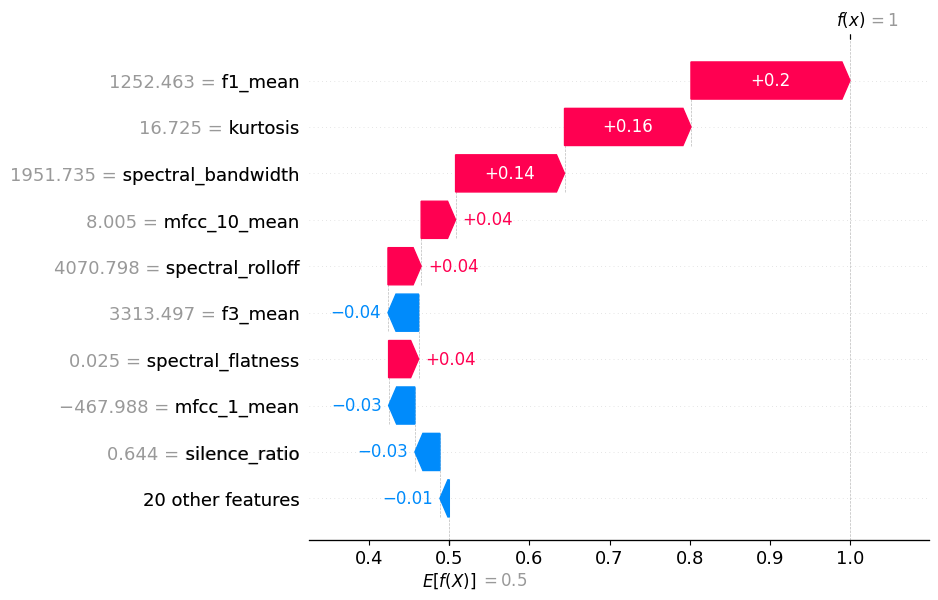
\includegraphics[width=\textwidth]{imagenes/pipe_shap_svm_local_2.png}
	\caption{Explicación local de SVM con SHAP para audios nuevos en español}
	\label{fig:pipe_shap_svm_esp_2}
\end{figure}

% Pipe SVM SHAP local ingles
\begin{figure}
	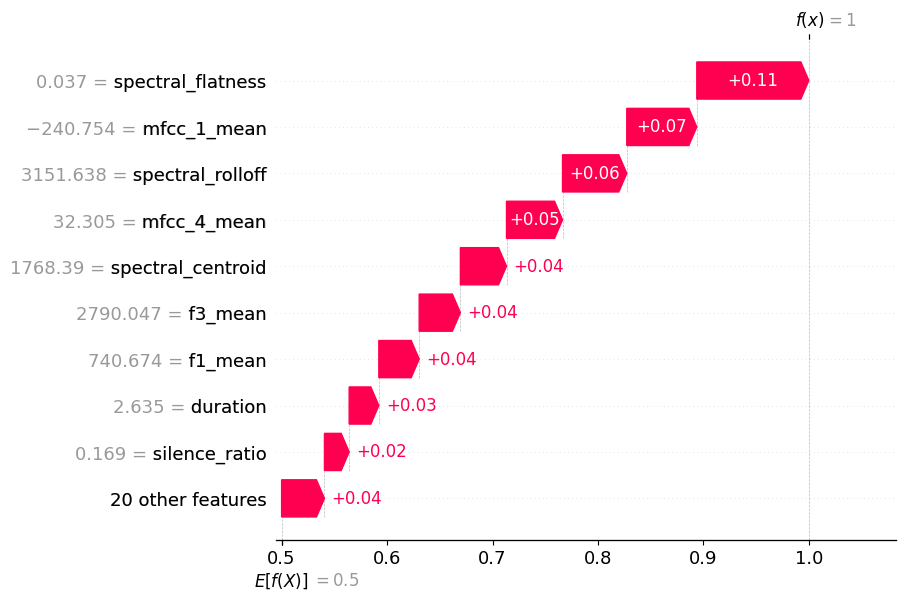
\includegraphics[width=\textwidth]{imagenes/pipe_shap_svm_local_eng_1.png}
	\caption{Explicación local de SVM con SHAP para audios nuevos en inglés}
	\label{fig:pipe_shap_svm_eng_1}
\end{figure}

\begin{figure}
	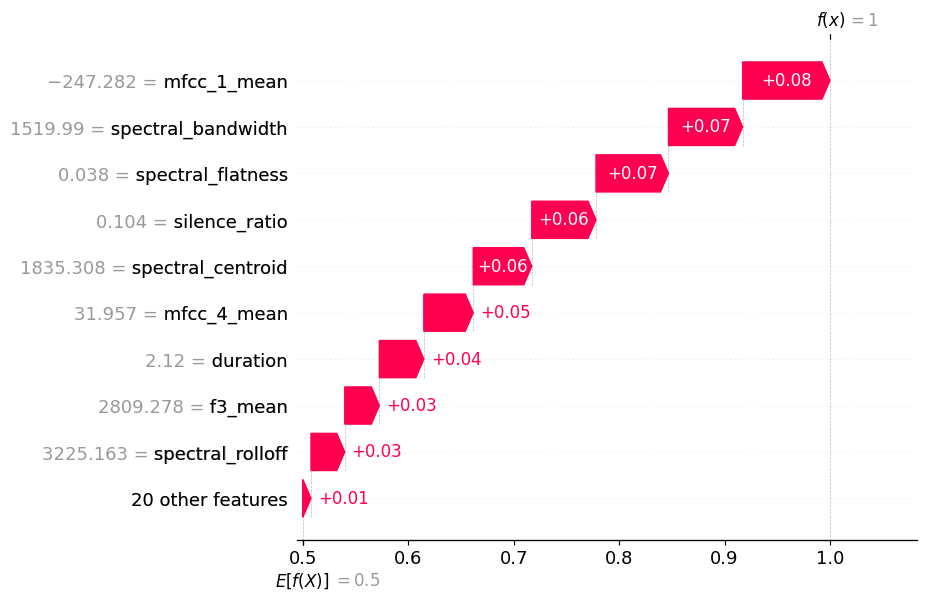
\includegraphics[width=\textwidth]{imagenes/pipe_shap_svm_local_eng_2.png}
	\caption{Explicación local de SVM con SHAP para audios nuevos en inglés}
	\label{fig:pipe_shap_svm_eng_2}
\end{figure}

% Pipe SVM SHAP global
\begin{figure}
	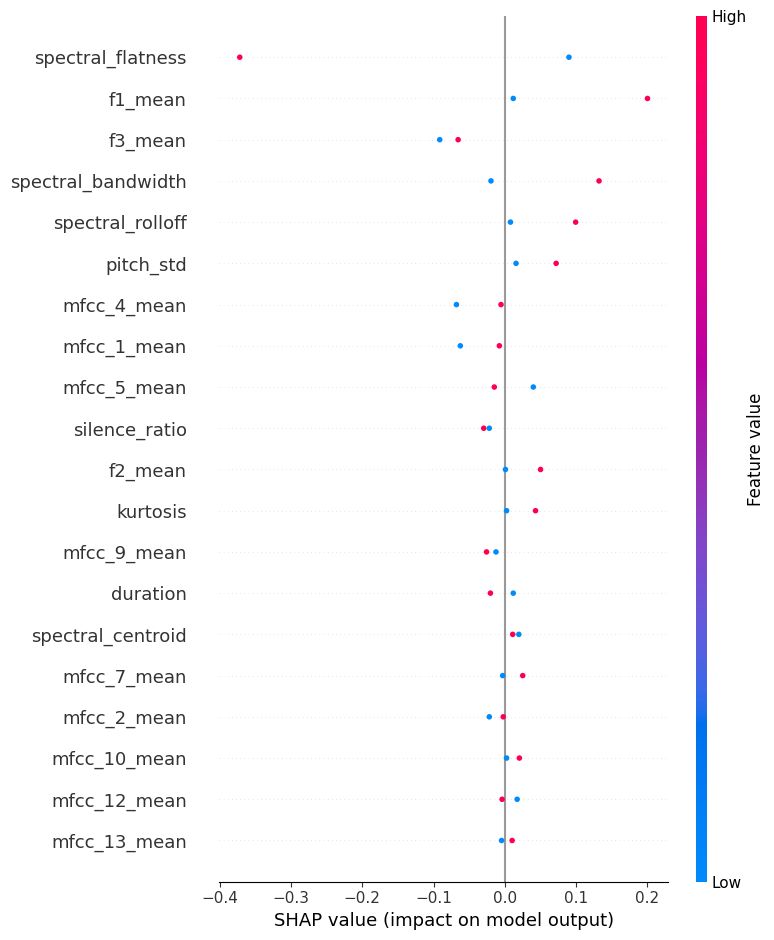
\includegraphics[width=\textwidth]{imagenes/pipe_shap_svm_global.png}
	\caption{Explicación global de SVM con SHAP}
	\label{fig:pipe_shap_svm_global}
\end{figure}

% Pipe SVM LIME
\begin{figure}
	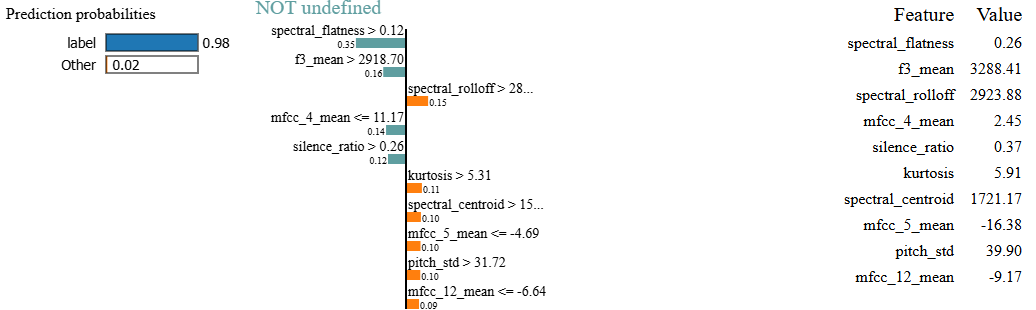
\includegraphics[width=\textwidth]{imagenes/pipe_lime_svm.png}
	\caption{Explicación local de SVM con LIME}
	\label{fig:pipe_lime_svm}
\end{figure}

\begin{figure}
    \centering
    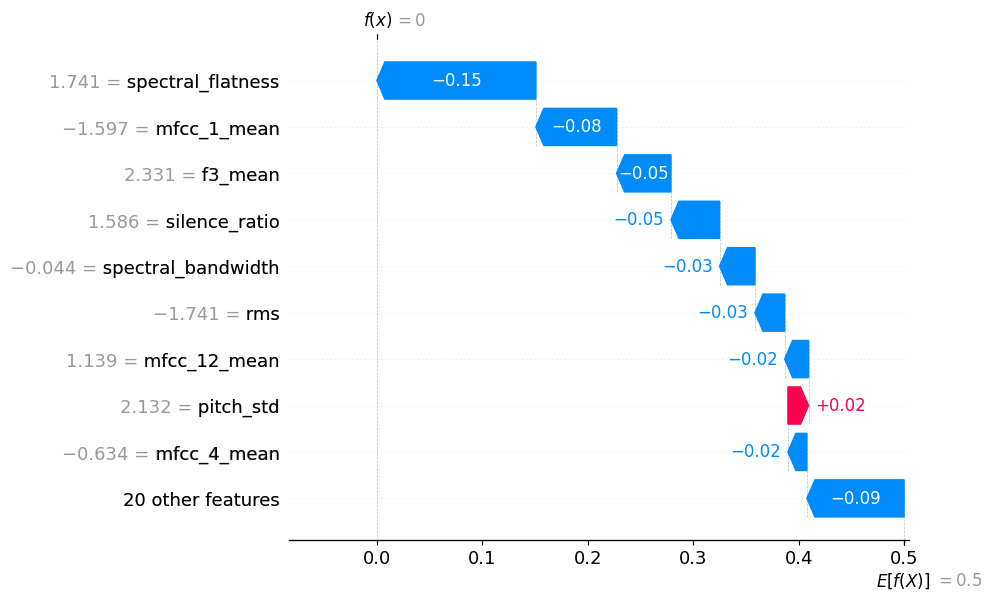
\includegraphics[width=\textwidth,height=\textheight,keepaspectratio]{imagenes/knn_shap_local.png}
    \caption{Explicación local de SHAP para el modelo KNN.}
    \label{fig:knn_shap_local}
\end{figure}

\begin{figure}
    \centering
    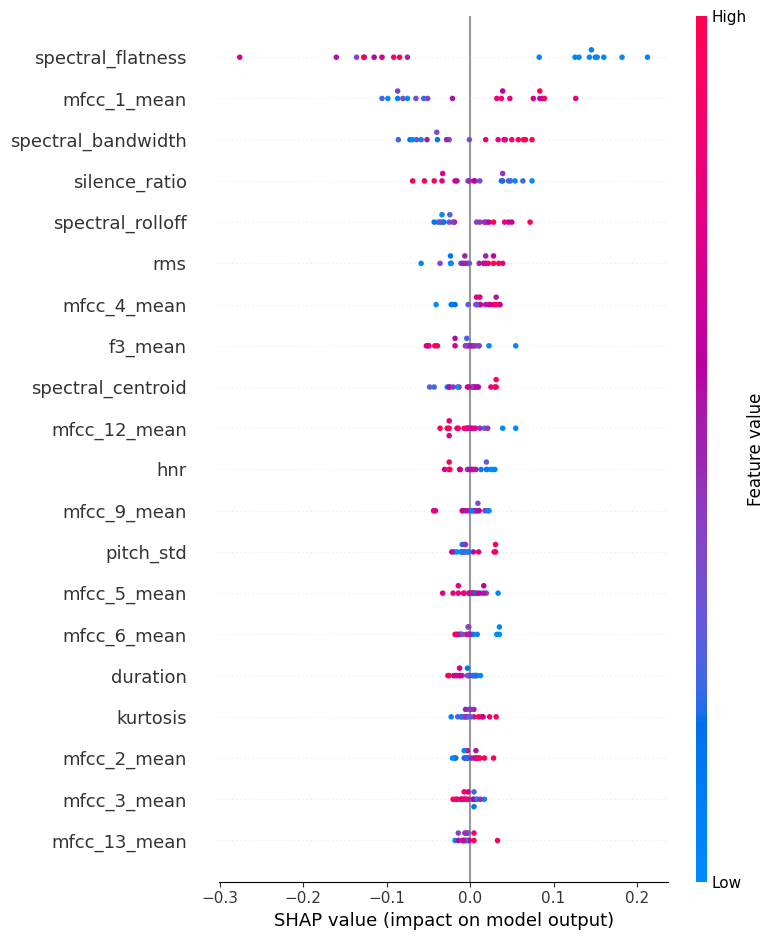
\includegraphics[width=\textwidth,height=\textheight,keepaspectratio]{imagenes/knn_shap_global.png}
    \caption{Importancia global de las características mediante SHAP para el modelo KNN.}
    \label{fig:knn_shap_global}
\end{figure}

\begin{figure}
    \centering
    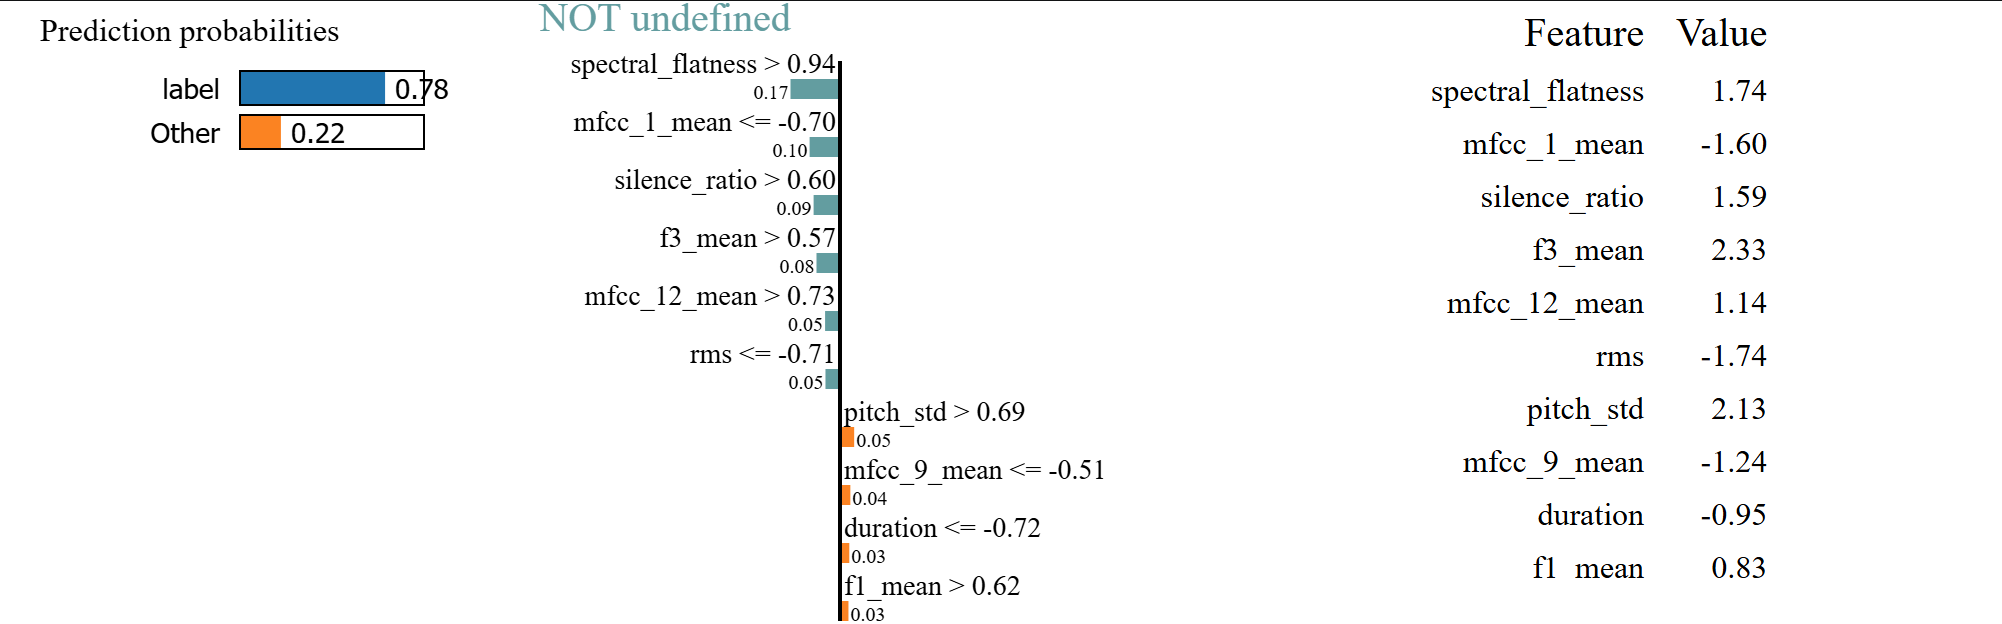
\includegraphics[width=\textwidth,height=\textheight,keepaspectratio]{imagenes/knn_lime.png}
    \caption{Explicación local generada por LIME para el modelo KNN.}
    \label{fig:knn_lime}
\end{figure}

\begin{figure}
    \centering
    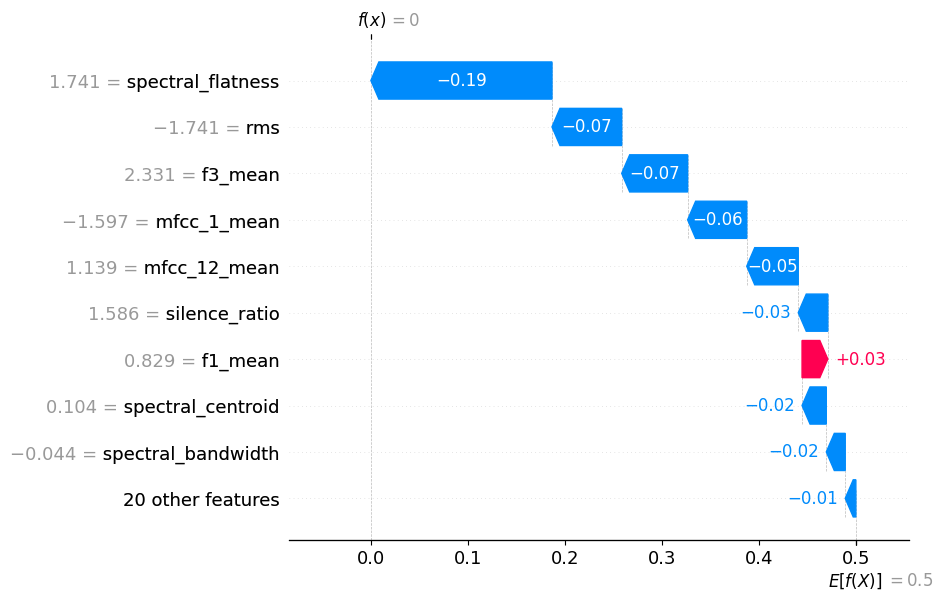
\includegraphics[width=\textwidth,height=\textheight,keepaspectratio]{imagenes/lr_shap_local.png}
    \caption{Explicación local de SHAP para el modelo de Regresión Logística.}
    \label{fig:lr_shap_local}
\end{figure}

\begin{figure}
    \centering
    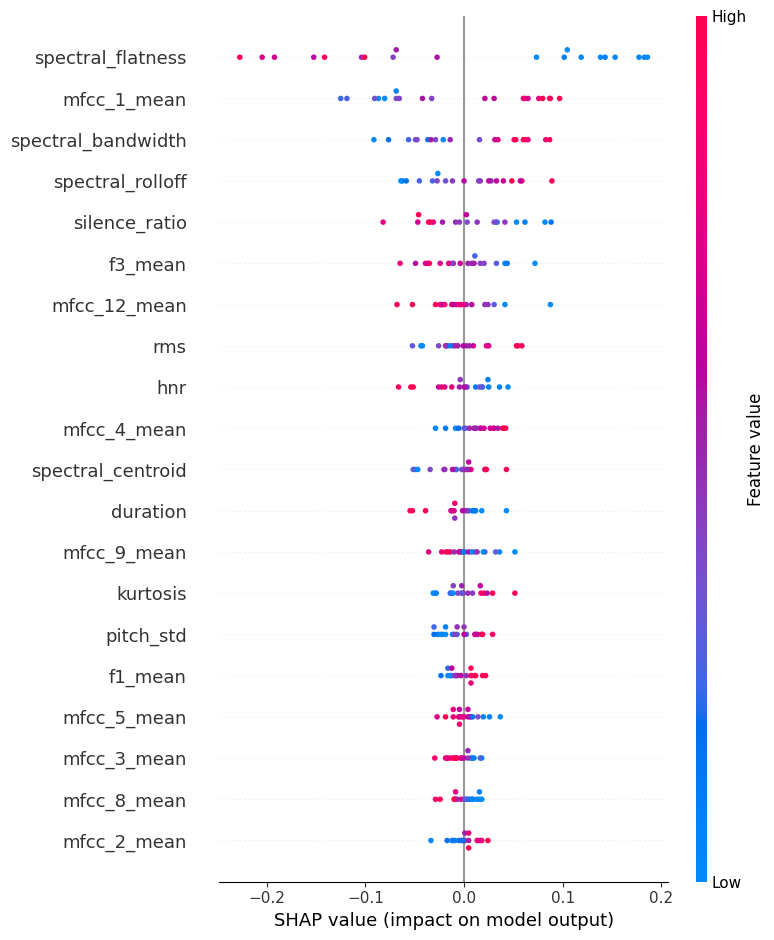
\includegraphics[width=\textwidth,height=\textheight,keepaspectratio]{imagenes/lr_shap_global.png}
    \caption{Importancia global de las características mediante SHAP para el modelo de Regresión Logística.}
    \label{fig:lr_shap_global}
\end{figure}

\begin{figure}
    \centering
    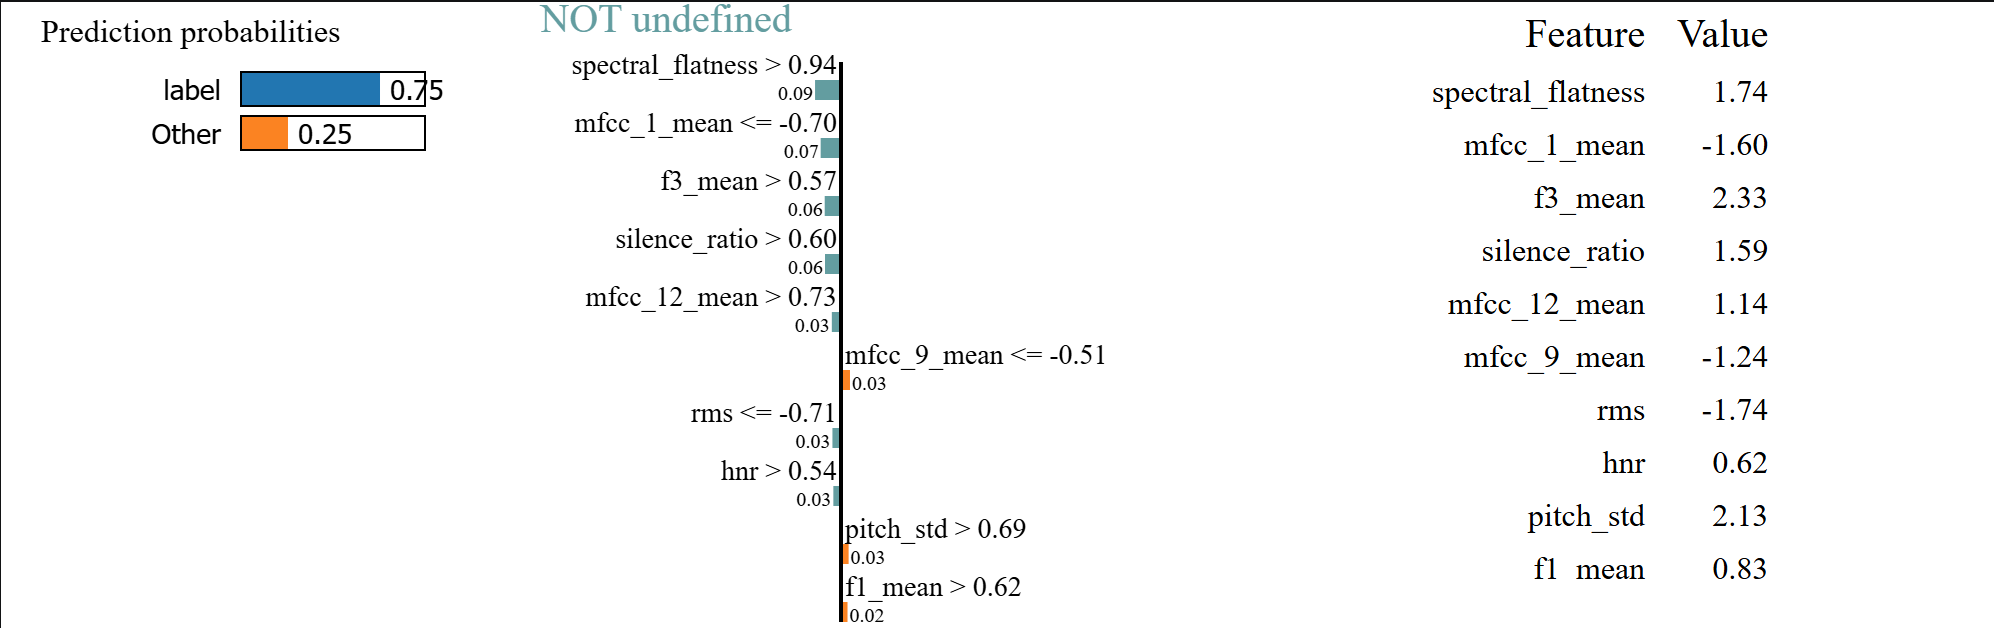
\includegraphics[width=\textwidth,height=\textheight,keepaspectratio]{imagenes/lr_lime.png}
    \caption{Explicación local generada por LIME para el modelo de Regresión Logística.}
    \label{fig:lr_lime}
\end{figure}

\begin{table}
\centering
\begin{tabular}{lccccccc}
\toprule
\textbf{Instancia} & \textbf{spectral flatness} & \textbf{mfcc 7 mean} & \textbf{mfcc 8 mean} & \textbf{mfcc 12 mean} & \textbf{skewness} & \textbf{kurtosis} & \textbf{Etiqueta} \\
\midrule
Counter factual 1 & -0.73109 & -1.87186 & -1.76405 & & -0.08304 & 2.90024 & 1 \\
Counter factual 2 & & & & -2.93504 & & & 1 \\
Counter factual 3 & -0.62483 & & & & -0.63265 & & 1 \\
\bottomrule
\end{tabular}
\caption{Counter factuals generados por DiCE para KNN (características principales)}
\label{tab:knn_dice}
\end{table}

\begin{table}
\centering
\begin{tabular}{lccccccc}
\toprule
\textbf{Instancia} & \textbf{spectral bandwidth} & \textbf{spectral rolloff} & \textbf{spectral flatness} & \textbf{mfcc 8 mean} & \textbf{mfcc 12 mean} & \textbf{kurtosis} & \textbf{Etiqueta} \\
\midrule
Counter factual 1 &  &  & -1.14511 & 0.24699 & -0.98900 & 1.34467 & 1 \\
Counter factual 2 & 2.22696 & 2.44032 &  &  & -3.07425 &  & 1 \\
Counter factual 3 & 1.17738 &  & -1.04455 &  & -0.58018 &  & 1 \\
\bottomrule
\end{tabular}
\caption{Counter factuals generados por DiCE para Regresión Logística}
\label{tab:lr_dice}
\end{table}